\subsection{Experiment 1: Static fabrics vs. \ac{mpc}}%
\label{sub:experiment_1_static_fabrics_vs_mpc}

In the first experiment, we compare the performance of an \ac{mpc}
formulation with \ac{sf}
\cite{Ratliff2020,Wyk2022}.
%
Compared to the formulation used in \cite{Spahn2021}, we use a workspace goal
rather than a configuration space goal, and apply a second order integration
scheme so that the control outputs are accelerations instead of velocities. We
clarify that the formulation deployed for the following tests is geometric as
the model used is a second order integrator and does not include the dynamics
of the robots. The main reason lies in the reduced computational costs and the
inaccessibility of a highly accurate model \cite{meo2021adaptation}.

\paragraph{Parameters}
The low-level controller of the robot runs at $1$ kHz. The fabrics are running at $100$ Hz
and the \ac{mpc} at $10$ Hz. The time horizon for the \ac{mpc}
planner was set to $T=3$s spread equally over
$H=30$ stages. Based on the findings in~\cite{Spahn2021}, we are confident that the \ac{mpc}
planner is close to its optimal settings. Moreover, we used the implementations
by~\cite{forcespro,forcesnlp}, which are reported to have improved performance over
open-source libraries like \textit{acado}.

\begin{figure}[h]
  \centering
  \begin{subfigure}{0.4\linewidth}
    \centering
    \includegraphics[height=4cm]{1_fabric_mpc/simPanda/fabric_20220223_102405_motion_in_frame}
    \caption{}%
    \label{subfig:experiment1_example}
  \end{subfigure}%
  \begin{subfigure}{0.6\linewidth}
    \centering
    \includegraphics[height=4cm]{3_moving_obstacles/simPanda/dynamicFabric_20220223_102854_motion_in_frame}
    \caption{}%
    \label{subfig:experiment3_example}
  \end{subfigure}
  \caption{Examples for simulation setups with \panda{}.
    Initial configuration are shown in white and final configurations in light green.
    Obstacles are visualized in red. In (a), only static obstacles are considered. In (b),
    the trajectories of two moving obstacles are visualized in light red.
  }%
  \label{fig:experiments_example}
\end{figure}

\paragraph{Simulation}
A series of $N=50$ runs was evaluated with the \panda{} in simulation. Randomized
end-effector positions were set for every run, while the initial configuration
remained unchanged. One to five spherical obstacles of
radius $r=0.15$ m were
placed in the workspace at random. An example setup is shown in
\cref{subfig:experiment1_example}. The results are summarized in 
\cref{fig:experiment1_simPanda}. Solver times with fabrics averaged at $1$ ms while the
\ac{mpc} solver took around $50$ ms in every time step. Although the path length is similar
with both solvers, the minimum clearance from obstacles is increased with \ac{sf}
($0.183$ m) compared to \ac{mpc} ($0.138$ m). This means that the trajectories are
safer and thus more suitable for dynamic environments.
Both motion generation methods fail in 6 cases. However, the \ac{sf} produce only
one collision while \ac{mpc} creates 5 collisions. The remaining failures are deadlocks.
For both methods, deadlocks result from local minima, highlighting the 
need for supportive global plans. Collisions are caused
by numerical inaccuracies, which are generally higher with \ac{mpc} due
to the lower frequency.

\begin{figure}[h]
  \centering
  \begin{subfigure}{1.0\linewidth}
    \centering
    \includegraphics[angle=-90,width=\textwidth]{1_fabric_mpc/simPanda/results_comparison}
    \caption{Metrics evaluation for successful experiments}%
    \label{subfig:experiment1_simPanda_res}
  \end{subfigure}
  \begin{subfigure}{1.0\linewidth}
    \centering
    \includegraphics[angle=-90,width=\textwidth]{1_fabric_mpc/simPanda/success}
    \caption{Success results}%
    \label{subfig:experiment1_simPanda_success}
  \end{subfigure}
  \caption{Results for randomized motion planning problems with the \panda{} in simulation.
    Lower values represent an improved performance of \ac{sf} over MPC.
    %Trajectory computed with optimization fabrics are more conservative and
    %computed in a decreased solver time.
  }%
  \label{fig:experiment1_simPanda}
\end{figure}

\paragraph{Real World}
For the experiments with the real robot, we limited the number of test runs to $N=20$. In
contrast to the simulated results, \ac{mpc} has significantly more collisions than
\ac{sf}, \cref{subfig:experiment1_realPanda_success}.  This is likely to be caused by the
lower frequency at which the \ac{mpc} is running. While in simulation the model matches
the actual behaviour perfectly and the time interval between two computations can be
accuratly predicted, more uncertainty in the model is present in the real world. This
leads to prediction errors that cause collisions.  For the collision free cases, the real
world experiments confirm that optimization fabrics tend to be more conservative with
respect to obstacles, see \textit{Clearance} in \cref{subfig:experiment1_realPanda_res}.
Similar to the simulated results, the solving time is reduced by a factor of around $50$
with fabrics. This
allows to run the planner at a higher frequency and thus generating smoother motions.

\begin{figure}[h]
  \centering
  \begin{subfigure}{\linewidth}
    \centering
    \includegraphics[angle=-90,width=\textwidth]{1_fabric_mpc/realPanda/results_comparison}
    \caption{Metrics evaluation for successful experiments}%
    \label{subfig:experiment1_realPanda_res}
  \end{subfigure}
  \begin{subfigure}{\linewidth}
    \centering
    \includegraphics[angle=-90,width=\textwidth]{1_fabric_mpc/realPanda/success}
    \caption{Success results}%
    \label{subfig:experiment1_realPanda_success}
  \end{subfigure}
  \caption{Results for randomized motion planning problems with the real \panda{}.
    \ac{sf} are more conservative around obstacles, improving on safety, while
    reducing the computational cost by a factor of $\approx$ 50.
    As a result of the increased clearance, collisions are more reliably avoided with
    \ac{sf}.
  }%
  \label{fig:experiment1_realPanda}
\end{figure}

\paragraph{Discussion}
The difference in performance (except for solver time) is likely caused by
the different objective metrics. The objective function in the \ac{mpc}
formulation is mainly governed by the Euclidean distance to the goal while
control inputs and velocity magnitude are given a relative small weight.
Avoidance behaviors, such as joint limit avoidance and obstacle avoidance,
are respected through inequality constraints. In contrast, \ac{sf} design the
objective in a purely geometric manner including all avoidance behaviors.
Thus the manifold for the motion is directly altered by the avoidance
behaviors, i.e., the manifold is \textit{bent} \cite{Ratliff2020} so that
the notion of shortest path changes with the addition of obstacles. This
shaping of the manifold leads to improved canvergence compared to the
combination of Euclidean distance objective function and inequality
constraints used with \ac{mpc}.
